\documentclass[tikz,border=10pt]{standalone}
\usepackage{tikz}
\usetikzlibrary{positioning,arrows.meta,shapes.geometric,fit,backgrounds,calc,decorations.pathreplacing}

\begin{document}
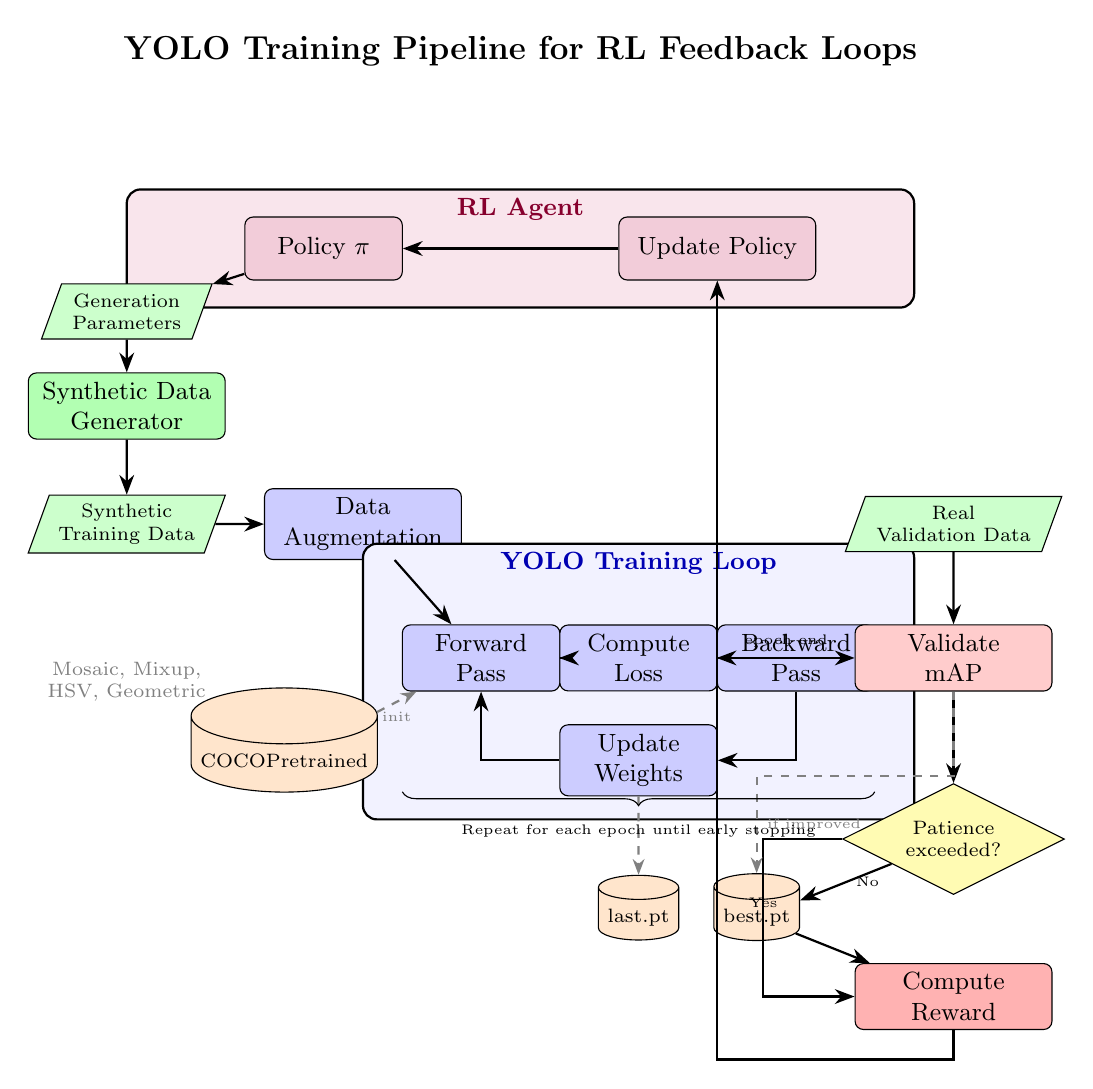
\begin{tikzpicture}[
    node distance=1cm and 1.5cm,
    every node/.style={font=\small},
    process/.style={rectangle, draw, fill=blue!20, minimum width=2.5cm, minimum height=0.8cm, align=center, rounded corners=3pt},
    data/.style={trapezium, trapezium left angle=70, trapezium right angle=110, draw, fill=green!20, minimum width=2cm, minimum height=0.7cm, align=center, font=\scriptsize},
    decision/.style={diamond, draw, fill=yellow!30, minimum width=1.5cm, minimum height=1cm, align=center, aspect=2, font=\scriptsize},
    checkpoint/.style={cylinder, draw, fill=orange!20, shape border rotate=90, minimum width=1cm, minimum height=0.6cm, aspect=0.3, font=\scriptsize},
    arrow/.style={-{Stealth[length=2.5mm]}, thick},
    dashedarrow/.style={-{Stealth[length=2mm]}, thick, dashed, gray},
    bigbox/.style={draw, thick, dashed, rounded corners=5pt, fill=#1, fill opacity=0.1}
]

% Title
\node[font=\bfseries\large] at (5,8.5) {YOLO Training Pipeline for RL Feedback Loops};

% === RL Agent Section (top) ===
\begin{scope}[shift={(0,6)}]
\node[draw, thick, fill=purple!10, rounded corners=5pt, minimum width=10cm, minimum height=1.5cm] (rlbox) at (5,0) {};
\node[font=\bfseries\small, purple!70!black] at (5,0.5) {RL Agent};
\node[process, fill=purple!20, minimum width=2cm] (rlpolicy) at (2.5,0) {Policy $\pi$};
\node[process, fill=purple!20, minimum width=2.5cm] (rlupdate) at (7.5,0) {Update Policy};
\end{scope}

% === Synthetic Data Generation ===
\node[process, fill=green!30] (syngen) at (0,4) {Synthetic Data\\Generator};
\node[data] (params) at (0,5.2) {Generation\\Parameters};

% === Training Data Flow ===
\node[data] (syndata) at (0,2.5) {Synthetic\\Training Data};
\node[process] (augment) at (3,2.5) {Data\\Augmentation};

% === Model Training Section ===
\begin{scope}
\node[draw, thick, fill=blue!5, rounded corners=5pt, minimum width=7cm, minimum height=3.5cm] (trainbox) at (6.5,0.5) {};
\node[font=\bfseries\small, blue!70!black] at (6.5,2) {YOLO Training Loop};

\node[process, minimum width=2cm] (forward) at (4.5,0.8) {Forward\\Pass};
\node[process, minimum width=2cm] (loss) at (6.5,0.8) {Compute\\Loss};
\node[process, minimum width=2cm] (backward) at (8.5,0.8) {Backward\\Pass};
\node[process, minimum width=2cm] (update) at (6.5,-0.5) {Update\\Weights};
\end{scope}

% === Pretrained Weights ===
\node[checkpoint] (pretrained) at (2,-0.5) {COCO\\Pretrained};

% === Validation Section ===
\node[data] (realval) at (10.5,2.5) {Real\\Validation Data};
\node[process, fill=red!20] (validate) at (10.5,0.8) {Validate\\mAP};

% === Early Stopping Decision ===
\node[decision] (earlystop) at (10.5,-1.5) {Patience\\exceeded?};

% === Checkpoints ===
\node[checkpoint] (bestpt) at (8,-2.5) {best.pt};
\node[checkpoint] (lastpt) at (6.5,-2.5) {last.pt};

% === Reward Computation ===
\node[process, fill=red!30] (reward) at (10.5,-3.5) {Compute\\Reward};

% === ARROWS ===

% RL to syngen
\draw[arrow] (rlpolicy) -- (params);
\draw[arrow] (params) -- (syngen);

% Syngen to training
\draw[arrow] (syngen) -- (syndata);
\draw[arrow] (syndata) -- (augment);
\draw[arrow] (augment) -- (forward);

% Pretrained to forward
\draw[dashedarrow] (pretrained) -- (forward) node[midway, below, font=\tiny] {init};

% Training loop
\draw[arrow] (forward) -- (loss);
\draw[arrow] (loss) -- (backward);
\draw[arrow] (backward) |- (update);
\draw[arrow] (update) -| (forward);

% Validation
\draw[arrow] (realval) -- (validate);
\draw[arrow] (loss) -- (validate) node[midway, above, font=\tiny] {epoch end};

% Early stopping
\draw[arrow] (validate) -- (earlystop);
\draw[arrow] (earlystop) -- node[right, font=\tiny] {No} (bestpt);
\draw[arrow] (earlystop.west) -- ++(-1,0) |- node[near start, above, font=\tiny] {Yes} (reward);

% Checkpoints
\draw[dashedarrow] (update) -- (lastpt);
\draw[dashedarrow] (validate) -- ++(0,-1.5) -| (bestpt) node[near end, right, font=\tiny] {if improved};

% Reward to RL
\draw[arrow] (reward) -- ++(0,-0.8) -| (rlupdate);
\draw[arrow] (rlupdate) -- (rlpolicy);

% Reward from best.pt
\draw[arrow] (bestpt) -- (reward);

% === Labels and annotations ===
\node[font=\scriptsize, align=center, gray] at (0,0.5) {Mosaic, Mixup,\\HSV, Geometric};

% Epoch counter annotation
\draw[decorate, decoration={brace, amplitude=5pt, mirror}] (3.5,-0.9) -- (9.5,-0.9);
\node[font=\tiny, below] at (6.5,-1.2) {Repeat for each epoch until early stopping};

\end{tikzpicture}
\end{document}
